%\appendix 
\refstepcounter{chapter} 
\chapter*{When Will the Rapture Take Place?}\index{Rapture} 
\markboth{Appendix~\thechapter\quad When Will the Rapture Take Place?}%
         {Appendix~\thechapter\quad When Will the Rapture Take Place?}
%\addcontentsline{toc}{chapter} {\protect\numberline{Appendix~\thechapter} When Will the Rapture Take Place?}
\addcontentsline{toc}{chapter} {\protect\numberline{\thechapter} When Will the Rapture Take Place?}




\section*{What Is the Rapture?}\index{Rapture}

The term \textit{Rapture\index{Rapture}} refers to the event in which believers are caught up to meet the Lord. The principal biblical passages are 1 Thessalonians 4:13--18 and 1 Corinthians 15:51--52.

In 1 Thessalonians 4:13--18, Paul assures believers that they need not grieve like those who have no hope. Just as Jesus died and rose again, so God will bring with Jesus those who have died in Him. When the Lord Himself descends from heaven, accompanied by a commanding shout, the voice of the archangel, and the trumpet call of God, the dead in Christ will rise first. Then those believers who are still alive will be caught up together with them in the clouds to meet the Lord in the air. From that moment onward, they will be with the Lord forever. Paul concludes by urging believers to encourage one another with these words (NIV).

Likewise, in 1 Corinthians 15:51--52, Paul reveals a mystery: not all believers will die, but all will be changed. In an instant, in the twinkling of an eye, at the last trumpet, the dead will be raised imperishable, and the living will be transformed (NIV).

Christians have proposed three principal views concerning the timing of the Rapture\index{Rapture}: 
\begin{itemize}
\item the pretribulation\index{Rapture!pretribulation view}, 
\item midtribulation\index{Rapture!midtribulation view}, and 
\item posttribulation\index{Rapture!posttribulation view} views. 
\end{itemize}
These positions represent different conclusions drawn by interpreters from the biblical passages as a whole.

\section*{The Pretribulation Rapture}\index{Rapture!pretribulation view}\index{Rapture}

The pretribulation\index{Rapture!pretribulation view} view holds that the church will be caught up to meet the Lord before the seven-year Great Tribulation\index{Great Tribulation} begins. It is because that several New Testament passages that promise believers deliverance from the wrath\index{wrath of God} to come.

\begin{itemize}
\item \textbf{1 Thessalonians 1:10:} Jesus is the one who rescues believers from the coming wrath.
\item \textbf{1 Thessalonians 5:9:} God has not appointed believers to suffer wrath but to receive salvation through the Lord Jesus Christ. The Greek word translated ``punishment'' in some Chinese renderings is the word for ``wrath.'' The surrounding passage (5:1--3) concerns the day of the Lord\index{day of the Lord}.
\item \textbf{Romans 5:9:} Having been justified by Christ's blood, believers will be saved from God's wrath through Him.
\item \textbf{Revelation 3:10:} Christ promises to keep His faithful people from the hour of trial that is coming upon the whole world. Advocates of the pretribulation\index{Rapture!pretribulation view} view understand this promise as protection from being present during that period, rather than preservation while passing through it.
\item \textbf{Luke 21:36:} Jesus calls His followers to remain watchful and pray, so that they may escape what is coming and stand before the Son of Man\index{Son of Man}.
\end{itemize}

The Old Testament also foreshadows God's deliverance of His people before judgment\index{judgment} falls:
\begin{itemize}
\item \textbf{Genesis 5:24:} Enoch was taken by God before the judgment of the Flood.
\item \textbf{Genesis 19:22:} Before judgment fell upon Sodom\index{Sodom}, the angel urged Lot to flee to the designated place, explaining that nothing could be done until he arrived there. The judgment was delayed until Lot had reached safety.
\end{itemize}

\begin{figure}[h]
    \centering
    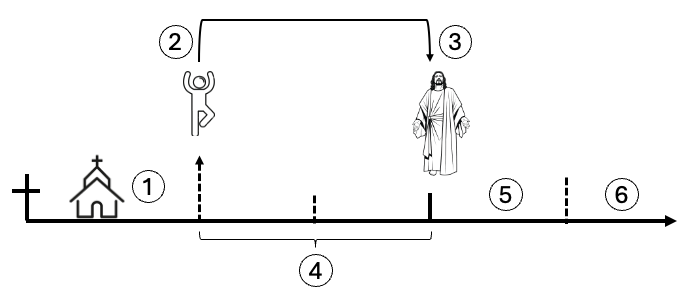
\includegraphics[
    width=1\textwidth,
    trim=0 0 0 0,
    clip]{images/pretribulation.png}
    \caption{The Pretribulation Rapture }
    \label{fig:pretribulation}
\end{figure}
The sequence of events in the pretribulation\index{Rapture!pretribulation view} view is illustrated in Figure~\ref{fig:pretribulation}: 
\begin{itemize}
\item[\ding{172} ] the Church Age; 
\item[\ding{173} ] the Rapture\index{Rapture} before the Great Tribulation\index{Great Tribulation};
\item[\ding{174} ] Christ's return to earth with His people to reign; 
\item[\ding{175} ] the Great Tribulation; 
\item[\ding{176} ] the Millennium\index{millennium}; 
\item[\ding{177} ] the new heaven and the new earth.
\end{itemize}



\section*{The Midtribulation Rapture}\index{Rapture!midtribulation view}\index{Rapture}

The midtribulation\index{Rapture!midtribulation view} view holds that the church will pass through the first three and a half years of the Great Tribulation\index{Great Tribulation} and then be caught up before God's wrath\index{wrath of God} is poured out in the latter half. Its proponents regard the midpoint of Daniel\index{Daniel}'s seventieth seven as a decisive turning point and connect the ``last trumpet'' mentioned by Paul with the seventh trumpet\index{trumpets, seven!7@seventh trumpet} in Revelation.

The principal passages cited in support of this view include the following:

\begin{itemize}
\item \textbf{Daniel 9:27:} In the middle of the seven, sacrifice and offering will cease. The midpoint of the seven-year period is therefore understood as a major dividing line in the prophetic sequence.
\item \textbf{1 Corinthians 15:52:} Paul says that believers will be changed at the last trumpet. Advocates of the midtribulation\index{Rapture!midtribulation view} view identify this trumpet with the seventh trumpet\index{trumpets, seven!7@seventh trumpet} in Revelation 11:15.
\item \textbf{Revelation 11:11--12:} After the two witnesses\index{two witnesses} have prophesied for 1,260 days\index{1,260 days}, they hear a voice from heaven calling, ``Come up here.'' They ascend to heaven in a cloud. Some interpreters regard this scene as a picture of the Rapture\index{Rapture} taking place in the middle of the Tribulation.
\item \textbf{Revelation 11:15, 18:} When the seventh angel sounds his trumpet, heaven announces that God's kingdom has come and that His wrath has arrived. Advocates of this view place the outpouring of divine wrath, particularly the seven bowls\index{bowls, seven} described in Revelation 16, in the latter half of the Tribulation.
\item \textbf{1 Thessalonians 5:9:} God has not appointed believers to suffer wrath. Midtribulation interpreters distinguish the persecution\index{persecution} inflicted by human powers and the Antichrist\index{Antichrist} during the first half from the outpouring of God's wrath during the second half. They therefore conclude that believers will be caught up before that wrath begins.
\item \textbf{2 Thessalonians 2:3--4:} Before the gathering of believers, the man of lawlessness must be revealed and exalt himself in the temple\index{temple} of God, proclaiming himself to be God. This is commonly associated by advocates of this view with the midpoint of the seven-year period and with the abomination of desolation mentioned in Matthew 24\index{Matthew 24}:15.
\end{itemize}

\begin{figure}[htbp]
    \centering
    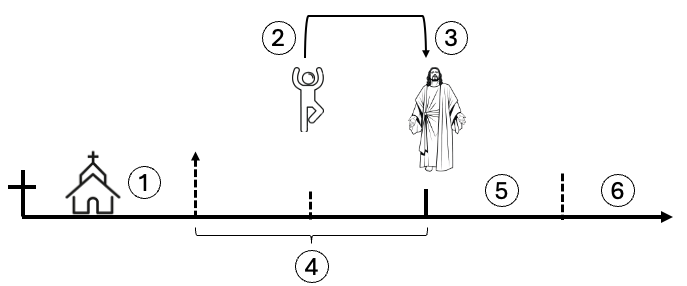
\includegraphics[
    width=1\textwidth,
    trim=0 0 0 0,
    clip]{images/midtribulation.png}
    \caption{The Midtribulation Rapture }
    \label{fig:midtribulation}
\end{figure}


The sequence of events in the midtribulation\index{Rapture!midtribulation view} view is illustrated in Figure~\ref{fig:midtribulation}: 
\begin{itemize}
\item[\ding{172} ] the Church Age; 
\item[\ding{173} ] the Rapture\index{Rapture} during the Great Tribulation\index{Great Tribulation};
\item[\ding{174} ] Christ's return to earth with His people to reign;
\item[\ding{175} ] the Great Tribulation; 
\item[\ding{176} ] the Millennium\index{millennium};
\item[\ding{177} ] the new heaven and the new earth.
\end{itemize}


\section*{The Posttribulation Rapture}\index{Rapture!posttribulation view}\index{Rapture}

The posttribulation\index{Rapture!posttribulation view} view holds that the church will pass through the Great Tribulation\index{Great Tribulation}. Believers will be caught up to meet the Lord in the air when Christ returns in glory\index{glory} at the end of that period. Proponents argue that the New Testament places the gathering of God's people after the Tribulation.

The principal passages cited in support of this view include the following:

\begin{itemize}
\item \textbf{Matthew 24\index{Matthew 24}:29--31:} Jesus says that immediately after the distress of those days, the Son of Man\index{Son of Man} will appear and send His angels with a loud trumpet call to gather His elect from the four winds. Advocates of the posttribulation\index{Rapture!posttribulation view} view understand this as clear evidence that the gathering of God's people takes place after the Tribulation.
\item \textbf{2 Thessalonians 2:1--3:} Paul speaks of the coming of the Lord Jesus Christ and the gathering of believers to Him. He then explains that the day will not come until the rebellion occurs and the man of lawlessness is revealed. This is understood to mean that the Antichrist\index{Antichrist} will appear before believers are gathered to the Lord.
\item \textbf{2 Thessalonians 1:6--7:} Paul assures those suffering persecution\index{persecution} that they will receive relief when the Lord Jesus is revealed from heaven with His mighty angels. Advocates of this view understand this relief as coming at Christ's public return in glory.
\item \textbf{1 Corinthians 15:52:} Paul's reference to the last trumpet is understood in connection with the trumpet call in Matthew 24:31, suggesting that the transformation and gathering of believers occur at Christ's visible return.
\item \textbf{Revelation 20:4--5:} Those who bore witness to Jesus and refused to worship\index{worship} the beast\index{beast} come to life in what John calls ``the first resurrection\index{first resurrection}.'' Interpreters who understand this resurrection as occurring after the Great Tribulation\index{Great Tribulation} conclude that the resurrection of believers, and thus the Rapture\index{Rapture}, takes place after the Tribulation as well.
\item \textbf{John 17:15:} Jesus does not ask the Father to take His disciples out of the world, but to protect them from the evil one. Advocates of the posttribulation view see here a pattern of divine preservation: God can guard His people through times of suffering without necessarily removing them from those circumstances.
\end{itemize}

Advocates of this view also point to Old Testament events that illustrate God's ability to preserve His people through judgment rather than remove them beforehand:

\begin{itemize}
\item \textbf{Genesis 7:1, 23:} Noah was not taken away before the Flood. Instead, he passed through it in the ark and was preserved by God.
\item \textbf{Exodus 8:22:} When God brought plagues\index{plagues} upon Egypt\index{Egypt}, the Israelites remained in the land, but God set apart the region of Goshen so that the plague would not fall upon His people there.
\end{itemize}


\begin{figure}[htbp]
    \centering
    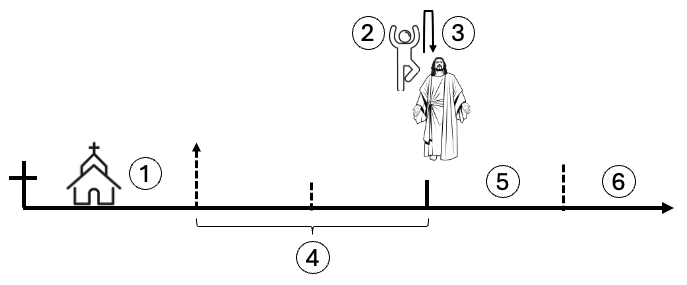
\includegraphics[
    width=1\textwidth,
    trim=0 0 0 0,
    clip]{images/posttribulation.png}
    \caption{The Posttribulation Rapture}
    \label{fig:posttribulation}
\end{figure}

The sequence of events in the posttribulation\index{Rapture!posttribulation view} view is illustrated in Figure~\ref{fig:posttribulation}: 
\begin{itemize}
\item[\ding{172} ] the Church Age; 
\item[\ding{173} ] the Rapture\index{Rapture} after the Great Tribulation\index{Great Tribulation}; 
\item[\ding{174} ] Christ's return to earth with His people to reign; 
\item[\ding{175} ] the Great Tribulation; 
\item[\ding{176} ] the Millennium\index{millennium}; 
\item[\ding{177} ] the new heaven and the new earth.
\end{itemize}

